%----------------------------------------------------------------------------------------
%    PACKAGES AND THEMES
%----------------------------------------------------------------------------------------

\documentclass[aspectratio=169,xcolor=dvipsnames]{beamer}
\setbeameroption{show notes} %TODO: Thomas a enlever avant la presentation
\usetheme{SimplePlus}

\useoutertheme{miniframes}  % Adds horizontal navigation dots at the top for subsections

\usecolortheme{} 

\setbeamercolor{block title}{bg=structure,fg=white}  % Navy blue background for block titles
\setbeamercolor{block body}{bg=structure!10,fg=structure}  % Light navy tint for block body

\definecolor{darkwine}{RGB}{128,0,32}  % Dark red wine
\newenvironment{errorblock}[1]{%
\begingroup%
\setbeamercolor{block title}{bg=darkwine,fg=white}%
\setbeamercolor{block body}{bg=structure!05,fg=black}%  % Very close to white background
\begin{block}{#1}%
}{\end{block}\endgroup}

\usepackage{comment}
\usepackage{hyperref}
\usepackage{graphicx} % Allows including images
\usepackage{booktabs} % Allows the use of \toprule, \midrule and \bottomrule in tables
\usepackage{array} % Allows >{\centering\arraybackslash} in tabular

% Define hyphenation command
\newcommand{\hyp}{-}

%----------------------------------------------------------------------------------------
%    TITLE PAGE
%----------------------------------------------------------------------------------------

\title{Diffusion Generative Flow Samplers: Improving Learning Signals Through Partial Trajectory Optimization}

\subtitle{Dinghuai Zhang*, Ricky T. Q. Chen, Cheng-Hao Liu, Aaron Courville \& Yoshua Bengio}
\author{Thomas Mousseau} 

% \institute
% {
%     Department of Computer Science and Information Engineering \\
%     National Taiwan University % Your institution for the title page
% }
\date{\today} % Date, can be changed to a custom date

%----------------------------------------------------------------------------------------
%    PRESENTATION SLIDES
%----------------------------------------------------------------------------------------

\begin{document}

\begin{frame}
    % Print the title page as the first slide
    \vspace*{-2cm}
    \titlepage
\end{frame}

\begin{frame}{Overview}
    % Throughout your presentation, if you choose to use \section{} and \subsection{} commands, these will automatically be printed on this slide as an overview of your presentation
    \tableofcontents
\end{frame}

%------------------------------------------------

\section{Introduction}

\subsection{Problem Statement}

\begin{frame}[t]{Generative Modeling}
\scriptsize
\begin{block}{Task}
    Sample from a complex (high-dimensional and multimodal) distribution $D$
\end{block}

$D$ can be given under the form of:

\begin{columns}[t]
\begin{column}{0.48\textwidth}
\begin{itemize}\itemsep2pt
    \item A dataset of samples $\{x_i\}_{i=1}^N \sim D$ (e.g., images, text, audio)
    \begin{figure}
        \centering
        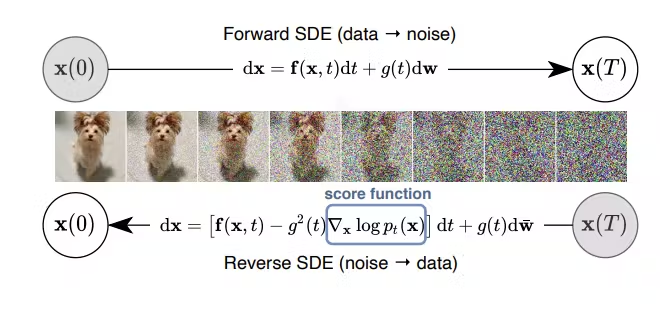
\includegraphics[width=0.9\textwidth]{figures/score_diffusion.png}
    \end{figure}
\end{itemize}
\end{column}
\begin{column}{0.48\textwidth}
\begin{itemize}\itemsep2pt
    \item An unnormalized density $\mu(x)$ where $D$ has density $\pi(x) \propto \mu(x)$ (e.g., 
    energy-based models, physics/chemistry)
    \begin{figure}
        \centering
        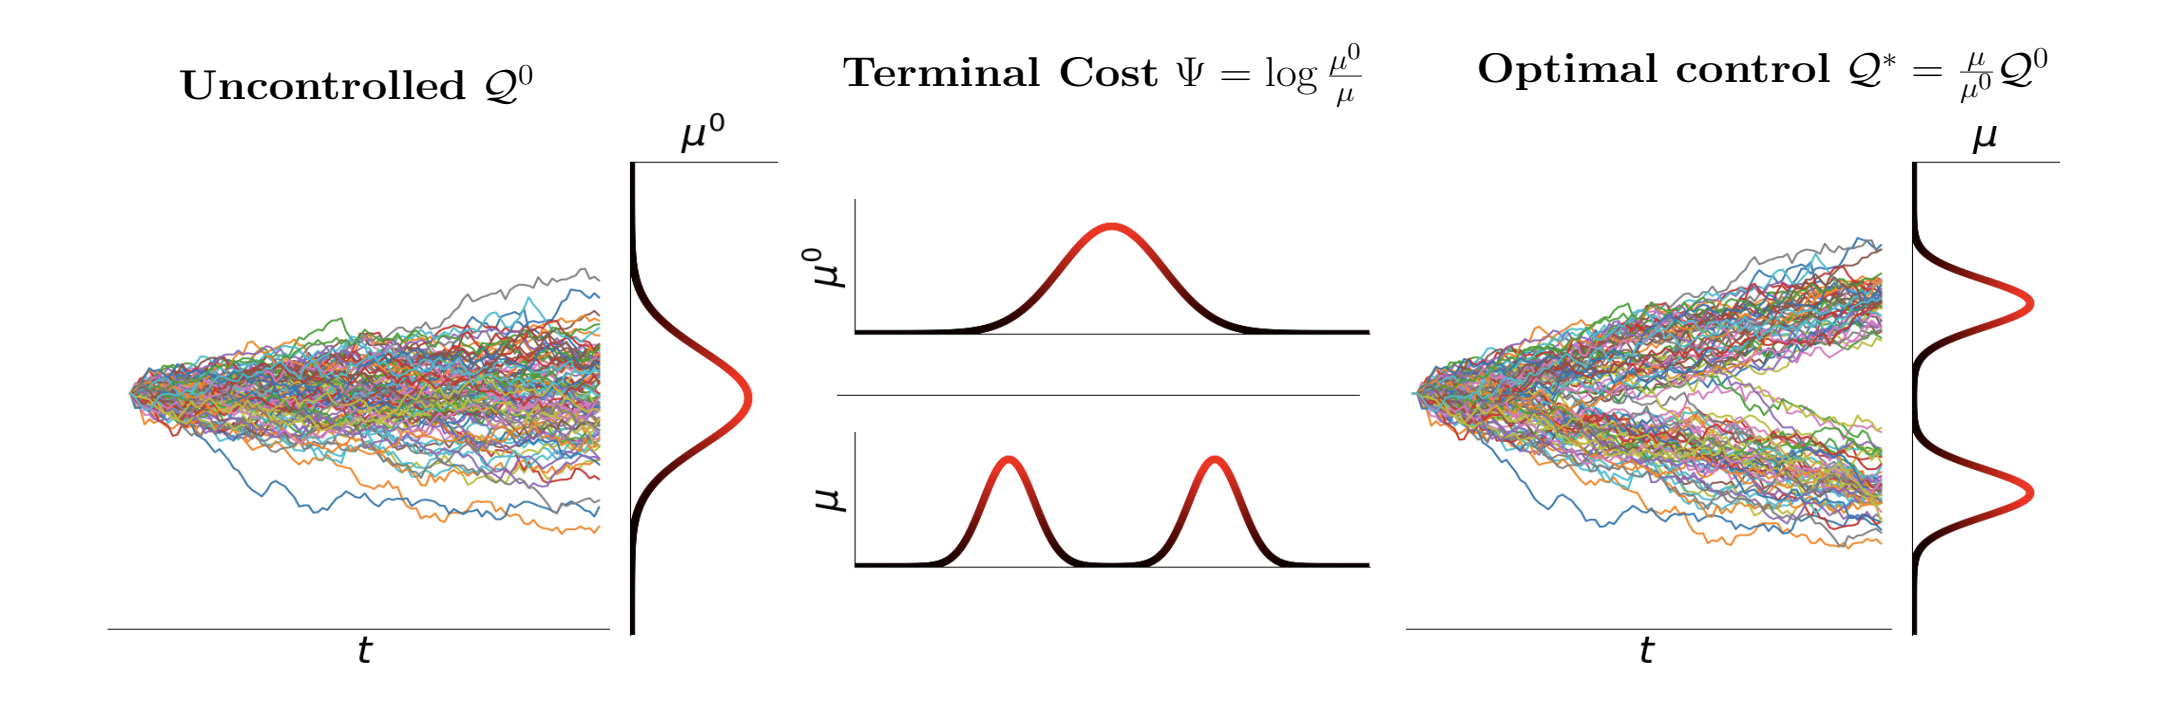
\includegraphics[width=0.9\textwidth]{figures/unconctrolled.png}
    \end{figure}
\end{itemize}
\end{column}
\end{columns}

\end{frame}

\begin{frame}[t]{Sampling from Unnormalized Densities}
\footnotesize
\textbf{Goal.} Sample from a $D$-dimensional target with unnormalized density $\mu(x)$ where $\mathbb R^D \to \mathbb R^+$.
\[
\pi(x)=\frac{\mu(x)}{Z},\qquad Z=\int_{\mathbb R^D}\mu(x)\,dx\ \text{(unknown)}.
\]
We assume we can evaluate $\mu(x)$, but we have no samples from $\pi$ and do not know $Z$.

\vspace{0.1cm}

\medskip
\textbf{Context.} We seek a \emph{sampler} (similar to MCMC/VI) that produces calibrated samples and, ideally, estimates of $\log Z$, \emph{without} any dataset from $\pi$.

\vspace{0.3cm}


\textbf{Chemistry (small-molecule conformers).} Different 3D conformations have a formation energy from force-field terms (bonds, angles, dihedrals, nonbonded); lower energy $\Rightarrow$ higher Boltzmann probability. A well-calibrated sampler is needed to draw conformers in proportion to these probabilities, which is important in binding-pose ranking/free-energy estimation, Boltzmann-weighted property prediction (e.g., NMR shifts), and generating diverse realistic 3D conformers for screening.
\end{frame}

\begin{frame}[t]{Diffusion Generative Flow Samplers}
\footnotesize
\textbf{Idea.} We will \emph{reframe sampling} from an unnormalized target $\pi(x)\propto \mu(x)$ as a \emph{stochastic optimal control (SOC)} problem: learn a control that steers a simple reference diffusion so its \emph{terminal marginal} matches $\pi$.

\medskip
\textbf{Why this helps.}
\begin{itemize}\itemsep2pt
  \item Gives a \emph{path-space} training objective/metric: a KL on trajectories $\mathrm{KL}(Q\,\|\,P)$ where $P$ is the reference paths reweighted by $\mu(x_T)$.
  \item The \emph{partition function $Z$ cancels} inside this objective, so we can train using only $\mu$ (and optionally $\nabla\log\mu$).
  \item Lets us optimize \emph{without samples from $\pi$} and still measure closeness to the true normalized endpoint.
\end{itemize}

\medskip
\textbf{Caveat (sets up DGFS).} This path-KL places supervision \emph{only at the terminal time} $\Rightarrow$ poor \emph{credit assignment} and high-variance gradients.

\medskip
\textbf{DGFS fix (preview).} Inject \emph{intermediate} learning signals via a GFlowNet-inspired \emph{learned flow} and \emph{subtrajectory balance}, enabling partial-trajectory training and more stable learning.
\end{frame}

\subsection{Stochastic Optimal Control}

% --- Slide 1 ---
\begin{frame}[t]{Steps 1--2: Forward \& Reference in \textit{discrete time}}
\footnotesize
\textbf{Controlled forward transition (learned drift).}
\[
P_F(x_{n+1}\mid x_n)\;=\;\mathcal N\!\big(x_{n+1};\;x_n + h\,f(x_n,n),\;h\sigma^2 I\big)
\]
\textbf{Controlled path law.}
\[
Q(x_{0:N})\;=\;p^{\text{ref}}_0(x_0)\;\prod_{n=0}^{N-1} P_F(x_{n+1}\mid x_n)
\]

\medskip
\textbf{Uncontrolled (reference) transition (zero drift).}
\[
P_F^{\text{ref}}(x_{n+1}\mid x_n)\;=\;\mathcal N\!\big(x_{n+1};\;x_n,\;h\sigma^2 I\big)
\]
\textbf{Reference path law and marginals.}
\[
Q^{\text{ref}}(x_{0:N})\;=\;p^{\text{ref}}_0(x_0)\;\prod_{n=0}^{N-1} P_F^{\text{ref}}(x_{n+1}\mid x_n),
\qquad p^{\text{ref}}_n(x)\;\text{is closed form.}
\]

\medskip
\textbf{Goal.} Learn $f$ so that the terminal marginal $Q(x_N)$ matches $\pi(x)=\mu(x)/Z$ (no data, $Z$ unknown).
\end{frame}

% --- Slide 2 ---
\begin{frame}[t]{Step 3: Path target \& KL $\Rightarrow$ SOC objective}
\scriptsize
% \textbf{Elementary identity: P(A,B) = P(A$\mid$B) P(B)}
% \[
% P(x_{0:N}) = P(x_{0:N-1} | x_N) P(x_N).
% \]

% \textbf{Reference bridge decomposition.}
% \[
% Q^{\text{ref}}(x_{0:N}) \;=\; Q^{\text{ref}}(x_{0:N-1}\mid x_N)\; p_N^{\text{ref}}(x_N),
% \qquad p_N^{\text{ref}}(x_N)=\!\int Q^{\text{ref}}(x_{0:N})\,dx_{0:N-1}.
% \]

\textbf{Target path measure via terminal reweighting.}
\[
P(x_{0:N}) \;\propto\; Q^{\text{ref}}(x_{0:N})\,\frac{\mu(x_N)}{p^{\text{ref}}_N(x_N)}
\qquad\Longrightarrow\qquad P(x_N)\propto\mu(x_N).
\]

\textbf{KL decomposition.}
\[
\mathrm{KL}(Q\|P)
=\mathbb E_{Q}\!\left[\log\frac{Q}{Q^{\text{ref}}}\right]
+\mathbb E_{Q}\!\left[\log\frac{p^{\text{ref}}_N(x_N)}{\pi(x_N)}\right].
\]
\medskip
\textbf{Running control cost (Gaussian mean-shift) Girsanov theorem.}
\[
\mathbb E_{Q}\!\left[\log\frac{Q}{Q^{\text{ref}}}\right]
=\mathbb E_Q \sum_{n=0}^{N-1}\frac{h}{2\sigma^2}\,\|f(x_n,n)\|^2.
\]

\textbf{Terminal potential from the target Girsanov theorem.}
\[
\mathbb E_{Q}\!\left[\log\frac{p^{\text{ref}}_N(x_N)}{\pi(x_N)}\right]
=\mathbb E_Q\!\big[\log p^{\text{ref}}_N(x_N)-\log \mu(x_N)\big]\;+\;\log Z.
\]

\end{frame}

\begin{frame}[t]{SOC objective}
\footnotesize
\medskip
\textbf{SOC objective (discrete-time).}
\[
\boxed{\ \min_{f}\ \mathbb E_Q\!\Big[\sum_{n=0}^{N-1}\tfrac{h}{2\sigma^2}\|f(x_n,n)\|^2\;+\;\log p^{\text{ref}}_N(x_N)-\log \mu(x_N)\Big]\ }
\]
\end{frame}


\begin{frame}[t]{Diffusion Process}
\scriptsize

\textbf{Idea.} Let the target “diffuse to Gaussian” via a reference process (VP/VE SDE). The \emph{reverse-time} dynamics can, in principle, generate target samples if we know the \emph{score} $\nabla_x \log p_t(x)$:
\[
\underbrace{dx_t=\sigma\,dW_t}_{\text{forward/noising}}
\quad\Longleftrightarrow\quad
\underbrace{dx_t=\big[f_{\text{ref}}(x,t)-\sigma^2\nabla_x \log p_t(x)\big]dt+\sigma\,d\bar W_t}_{\text{reverse/generative}}.
\]

\textbf{What is score matching?} 
Learn a network $s_\theta(x,t)\approx \nabla_x\log p_t(x)$ by regressing on \emph{noised data}:
\[
\min_\theta\ \mathbb E_{t}\,\mathbb E_{x_0\sim p_{\text{data}}}\,\mathbb E_{\varepsilon}\!
\big\|s_\theta(x_t,t)-\nabla_x\log p_t(x_t)\big\|^2,
\]
which is equivalent to denoising a corrupted sample $x_t$ back toward $x_0$.

\vspace{0.1cm}
\begin{errorblock}{Why Denoising Score Matching is \emph{not} applicable here}
\begin{itemize}\itemsep2pt
  \item We have \emph{no dataset} from $\pi$, only the unnormalized $\mu(x)$ (and maybe $\nabla\log\mu$).

\end{itemize}
\end{errorblock}

\end{frame}

\begin{frame}[t]{Alternative to DSM: learn the vector field (control)}
\scriptsize
\textbf{Reverse SDE drift (generative side).}
\[
dx_t=\big[f_{\text{ref}}(x,t)-\sigma^2\,\nabla_x \log p_t(x)\big]\,dt+\sigma\,d\bar W_t.
\]

\textbf{DSM route (data world).} Learn the \emph{score} $s_\theta(x,t)\approx\nabla_x\log p_t(x)$ from noised \emph{data}, then plug it into the reverse drift.

\textbf{Vector-field route (our setting).} Directly learn the \emph{control/drift} $u_\theta(x,t)$ instead of the score. The two are \emph{equivalent} via:
\[
u_\theta(x,t)\;=\;f_{\text{ref}}(x,t)\;-\;\sigma^2\,s_\theta(x,t)
\quad\Longleftrightarrow\quad
s_\theta(x,t)\;=\;\tfrac{f_{\text{ref}}(x,t)-u_\theta(x,t)}{\sigma^2}.
\]

\textbf{Why do this here?}
\begin{itemize}\itemsep2pt
  \item We have no dataset from $\pi$, so DSM can’t form expectations over $p_t$; scores $\nabla\log p_t$ are unavailable.
  \item Instead, treat $u_\theta$ as a \emph{control} and \emph{learn it} by minimizing a $Z$-free \textit{path-space} KL that uses only the given $\mu(\cdot)$.
  \item This sets up diffusion samplers à la PIS/DDS and enables DGFS’s improvements (intermediate, subtrajectory credit).
\end{itemize}

\textbf{Notation tip.} Use $u_\theta$ (or $f$) for the vector field to avoid clashing with $\mu(\cdot)$, which denotes the unnormalized density.
\end{frame}


\begin{frame}[t]{Sampling as a Stochastic Optimal Control problem}
\footnotesize
\textbf{Forward (controlled) process $Q$.} A Markov chain with Gaussian transitions:
\[
Q(x_{0:N}):\quad x_0\sim p_0^{\text{ref}},\quad x_{n+1}\sim P_F(\cdot\mid x_n)=\mathcal N\!\big(x_n + h\,f(x_n,n),\; h\sigma^2 I\big).
\]

\textbf{Reference process $Q^{\text{ref}}$.} Same covariance, zero drift:
\[
x_{n+1}\sim P_F^{\text{ref}}(\cdot\mid x_n)=\mathcal N\!\big(x_n,\; h\sigma^2 I\big),\qquad x_0\sim p_0^{\text{ref}},\ \ p_n^{\text{ref}}\text{ known.}
\]

\textbf{Target process $P$.} Tie the terminal marginal to $\pi$ via the reference:
\[
P(x_{0:N})\ :=\ Q^{\text{ref}}(x_{0:N})\;\frac{\pi(x_N)}{p_N^{\text{ref}}(x_N)}.
\]
Then $P(x_N)\propto \mu(x_N)$, making $P$ a valid path-space target.
\end{frame}

\begin{frame}[t]{Sampling as a Stochastic Optimal Control problem}
\footnotesize

\medskip
\textbf{Learning objective (discrete-time SOC).} Learn $f$ by minimizing the path KL:
\[
\min_{f}\ D_{\mathrm{KL}}(Q\ \|\ P)
\;\;\Longleftrightarrow\;\;
\min_{f}\ \mathbb E_{Q}\!\Big[\sum_{n=0}^{N-1}\frac{h}{2\sigma^2}\,\|f(x_n,n)\|^2\;+\;\log\Psi(x_N)\Big],
\]
with \(\Psi(x_N)=\dfrac{p_N^{\text{ref}}(x_N)}{\mu(x_N)}\).
(Continuous-time limit recovers the classic VE-SDE SOC formulation.)
\end{frame}





%------------------------------------------------
\section{Methodology}

\subsection{DGFS framework}


%------------------------------------------------
\section{Results and Limitations}

\subsection{Results}


%------------------------------------------------
\section{Conclusion}

\subsection{Key Insights}
% Add content: Summarize DGFS's impact and paper's contributions.

\subsection{Future Directions and Usage since its release}
% Add content: Discuss limitations, extensions, and personal thoughts.

\begin{frame}{Conclusion}

\end{frame}


\end{document}